\section{Requisiti Funzionali}

\subsection{Requisiti di Sistema} \label{Requisiti di Sistema}

\begin{enumerate}[start=1,label=\textbf{RF\theenumi}, labelwidth=4em, left=0pt, labelsep=1em, align=left]

    \item \label{itm:RF1} Il sistema EcoTrack deve essere costituito una \textbf{mobile app} e una \textbf{web app}.
    
    \item \label{itm:RF2} Il sistema deve avere 4 tipologie di utenti:
    \begin{itemize}
        \item Utente Anonimo (\textbf{non registrato})
        \item Cittadino (\textbf{registrato})
        \item Operatore Ecologico (\textbf{registrato})
        \item Amministratore (\textbf{registrato})
    \end{itemize}
    
\end{enumerate}

\subsubsection{Requisiti Mobile App}

\begin{enumerate}[start=3,label=\textbf{RF\theenumi}, labelwidth=4em, left=0pt, labelsep=1em, align=left]
    
    \item \label{itm:RF3} La mobile app deve essere composta da una schermata principale dove poter \textbf{selezionare un servizio} ed eventualmente \textbf{accedere} o \textbf{registrarsi}.
    
    \item \label{itm:RF4} La mobile app  deve fornire le funzionalità presenti in \hyperref[fig:mobileapp]{Figura 2}.
    
    \item \label{itm:RF5}   In riferimento al \hyperref[itm:RF4]{RF4}, nella sezione \textbf{Mappa Interattiva}, l'utente deve poter:
    \begin{itemize}
        \item Vedere i \textbf{cassonetti} sulla mappa e consultarne il livello di riempimento.
        \item Vedere i \textbf{cestini} sulla mappa e consultarne il livello di riempimento.
        \item Vedere i \textbf{punti di raccolta temporanei} per i rifiuti speciali (pile, olio, ... ), consultarne il livello di riempimento ed il tempo di permanenza in quel punto.
        \item Vedere la pianificazione della \textbf{pulizia stradale} (orari e vie interessate).
        \item Vedere la posizione e gli orari di apertura degli \textbf{ecocentri}.
    \end{itemize}
    
    \item \label{itm:RF6}   In riferimento al \hyperref[itm:RF4]{RF4}, nella sezione \textbf{Promemoria Raccolta}, l'utente deve poter:
    \begin{itemize}
        \item Consultare il \textbf{calendario} di raccolta rifiuti.
        \item Selezionare la \textbf{zona} dell'utente ed attivare le \textbf{notifiche} della raccolta porta a porta.
    \end{itemize}
    
    \item \label{itm:RF7}   In riferimento al \hyperref[itm:RF4]{RF4}, nella sezione \textbf{Segnalazioni}, l'utente deve poter:
    \begin{itemize}
        \item Inviare un \textbf{messaggio} di segnalazione in merito a situazioni di sporcizia, per sollecitare l'intervento della nettezza urbana.
        \item Allegare \textbf{materiale multimediale} in merito alle segnalazioni di cui sopra.
    \end{itemize}
        
    \item \label{itm:RF8}   In riferimento al \hyperref[itm:RF4]{RF4}, nella sezione \textbf{Prenota Smaltimento}, l'utente deve poter:
    \begin{itemize}
        \item \textbf{Prenotare} uno slot temporale in un ecocentro per il conferimento rifiuti.
        \item \textbf{Cancellare} un'eventuale prenotazione effettuata in precedenza.
    \end{itemize}

    \item \label{itm:RF9}   In riferimento al \hyperref[itm:RF4]{RF4}, nella sezione \textbf{Simula Tasse}, l'utente deve poter:
    \begin{itemize}
        \item \textbf{Selezionare} un metodo di calcolo della TARI, tra classico (applicato attualmente in Italia) e nordico (applicato nei paesi nordici).
        \item \textbf{Inserire i parametri} necessari per il calcolo della TARI.
    \end{itemize}

\end{enumerate}

\subsubsection{Requisiti Web App}

\begin{enumerate}[start=10,label=\textbf{RF\theenumi}, labelwidth=4em, left=0pt, align=left, itemindent=-0.6em]
    
    \item \label{itm:RF10} La web app deve essere composta da una schermata principale dove poter selezionare un
    \textbf{servizio di gestione} del sistema.
    
    \item \label{itm:RF11} La web app  deve fornire le funzionalità presenti in \hyperref[fig:webapp]{Figura 3}.

    \item \label{itm:RF12}   In riferimento al \hyperref[itm:RF11]{RF11}, nella sezione \textbf{Gestione Utenti}, l'utente deve poter:
    \begin{itemize}[itemindent=-0.6em]
        \item \textbf{Visualizzare }gli utenti.
        \item \textbf{Modificare} gli utenti.
        \item \textbf{Rimuovere} gli utenti.
        \item Modificare e conferire \textbf{permessi}.
    \end{itemize}
    
    \item \label{itm:RF13}   In riferimento al \hyperref[itm:RF11]{RF11}, nella sezione \textbf{{Gestione Smaltimento}}, l'utente deve poter:
    \begin{itemize}[itemindent=-0.6em]
        \item Supervisionare le richieste di smaltimento.
        \item Supervisionare lo stato degli ecocentri.
    \end{itemize}
        
    \item \label{itm:RF14}   In riferimento al \hyperref[itm:RF11]{RF11},  nella sezione \textbf{{Statistiche}}, l'utente deve poter:
    \begin{itemize}[itemindent=-0.6em]
        \item Visionare i \textbf{dati} relativi alla situazione ecologica attuale.
        \item Effetuare \textbf{analisi statistiche} sui dati.
    \end{itemize}

    \item \label{itm:RF15}   In riferimento al \hyperref[itm:RF11]{RF11}, nella sezione \textbf{{Impostazioni}}, l'utente deve poter configurare e gestire le opzioni di sistema.
    
\end{enumerate}

\begin{figure}[H]
    \centering
    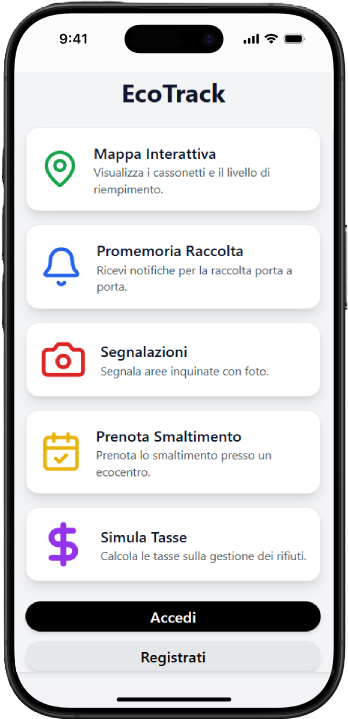
\includegraphics[width=0.27\linewidth]{D1-G1//Img/MobileApp.PNG}
    \caption{Prototipo Mobile App}
    \label{fig:mobileapp}
\end{figure}

\begin{figure}[H]
    \centering
    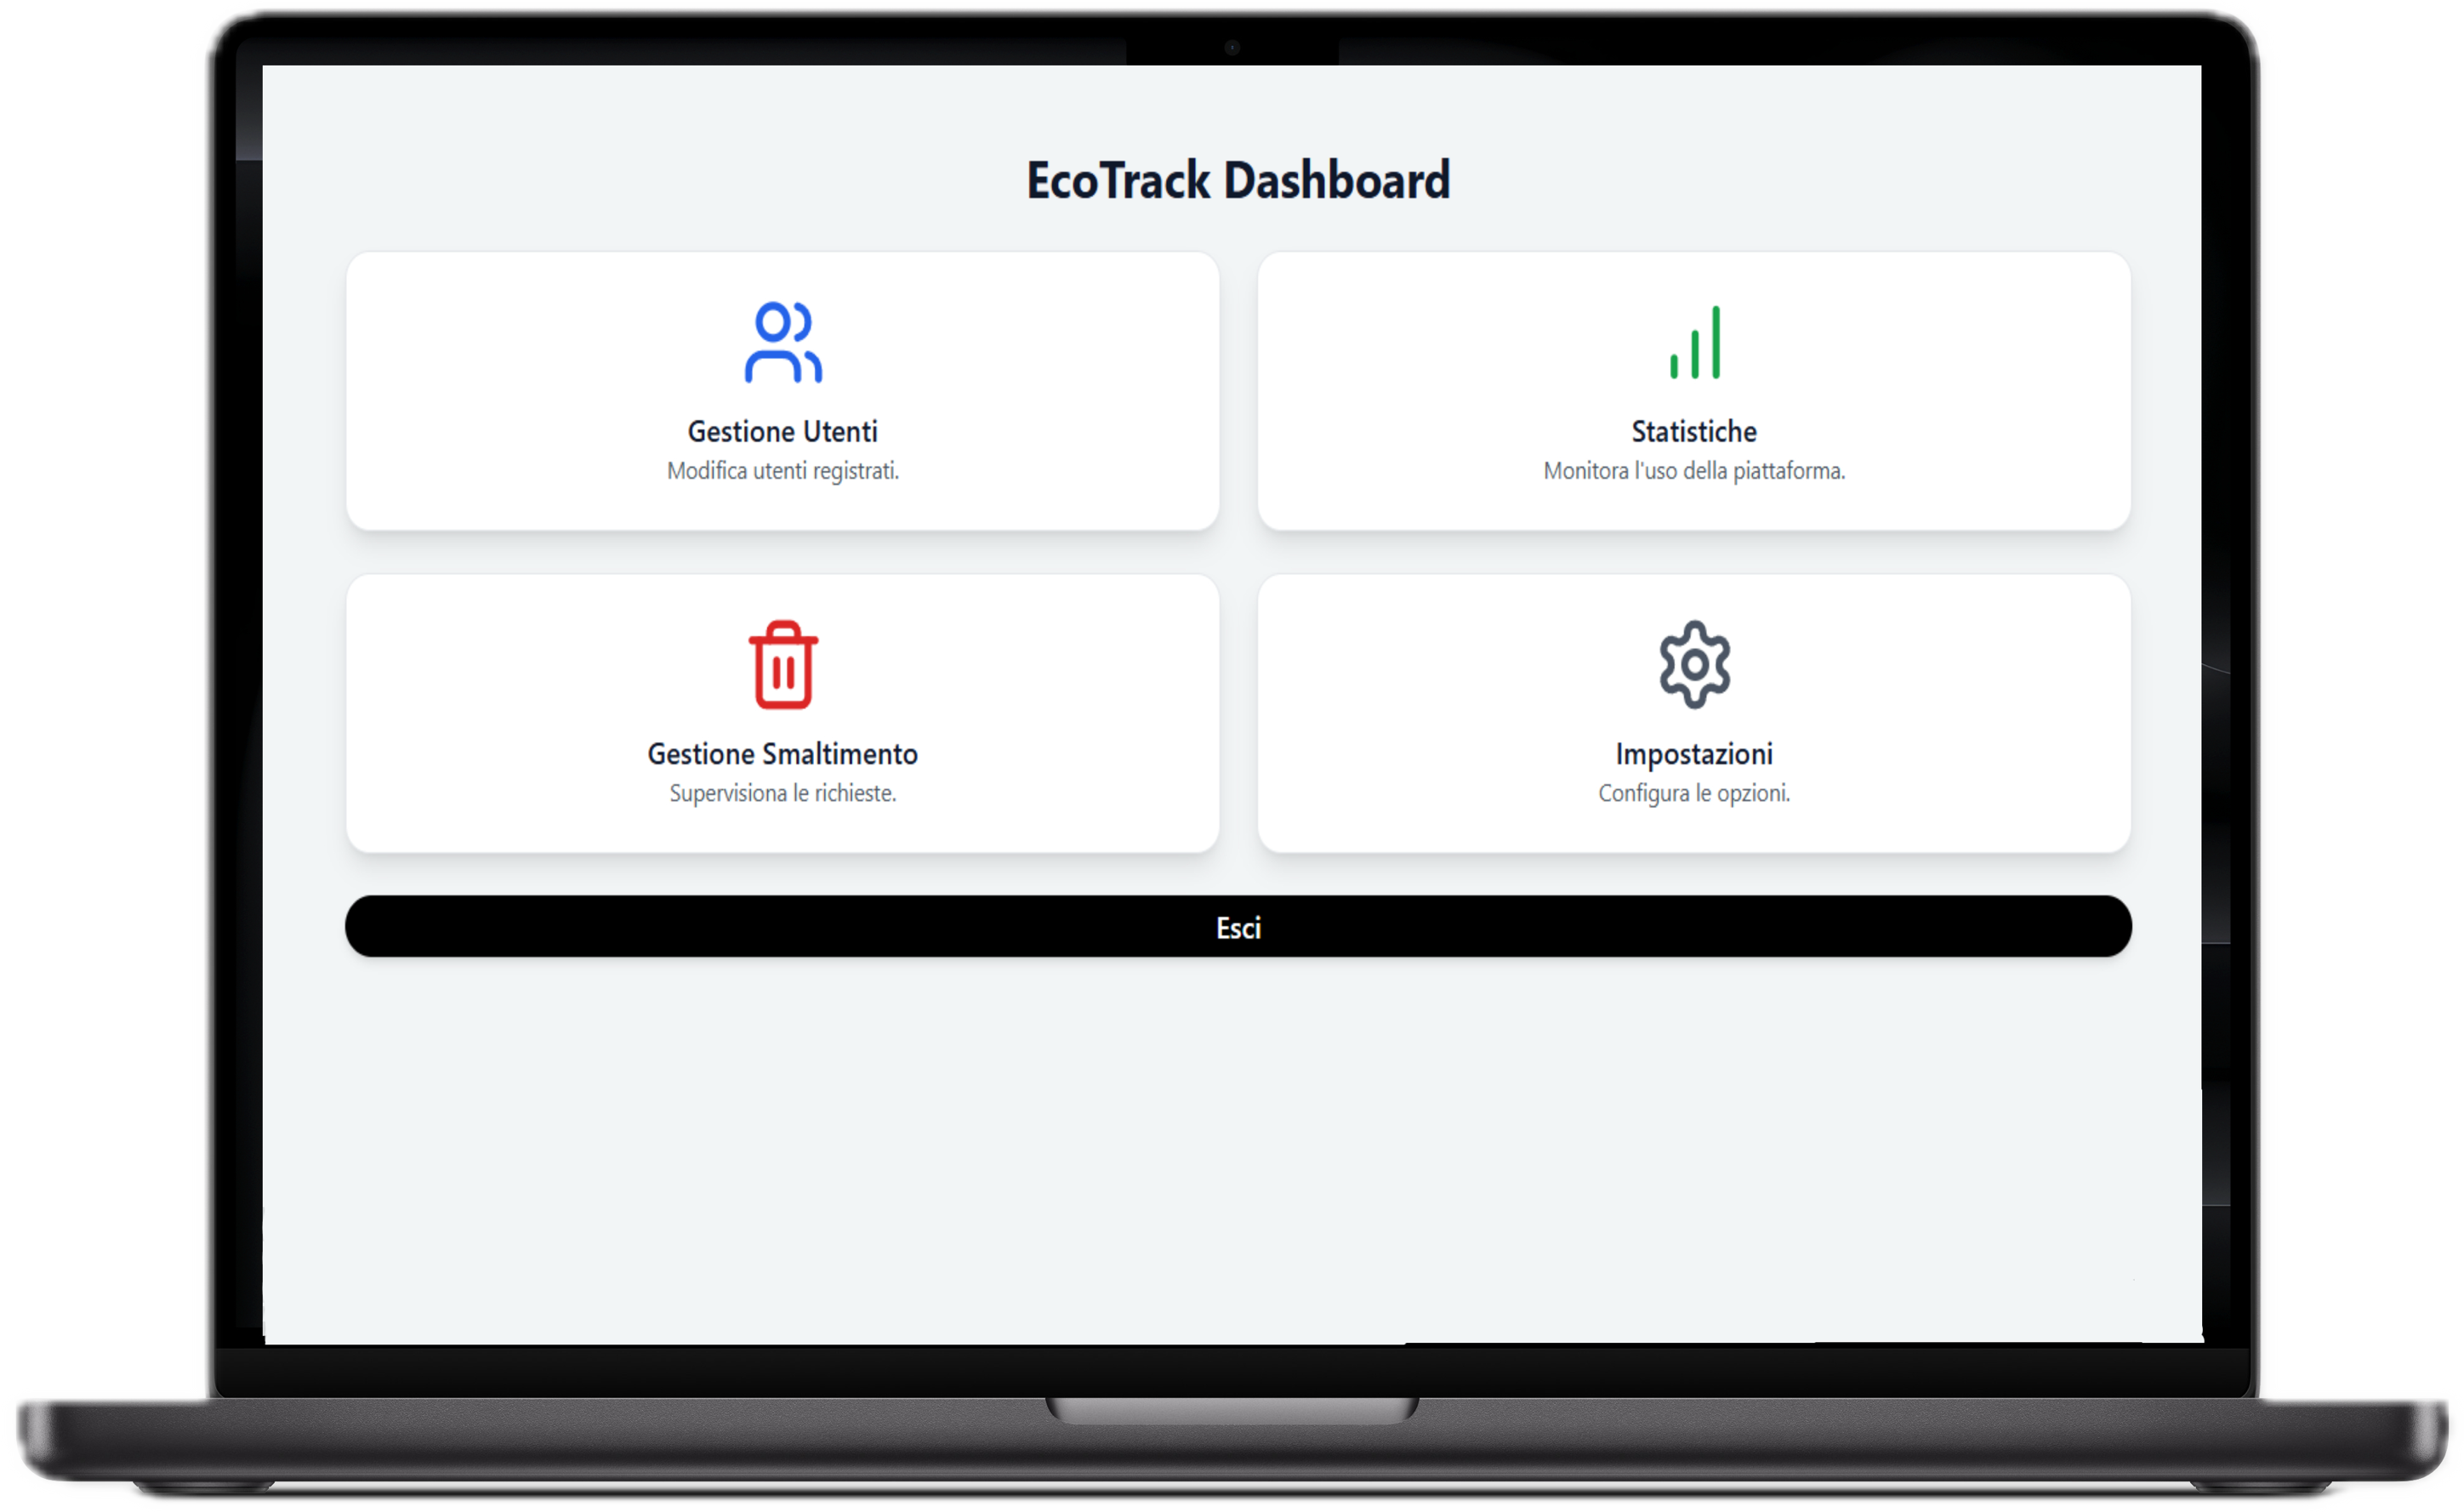
\includegraphics[width=0.73\linewidth]{D1-G1//Img/WebApp.png}
    \caption{Prototipo Web App}
    \label{fig:webapp}
\end{figure}

\subsection{Requisiti per Utenti}
\subsubsection{Utente Anonimo}

\begin{enumerate}[start=16,label=\textbf{RF\theenumi}, labelwidth=4em, left=0pt, align=left, itemindent=-0.6em]
    \item \label{itm:RF16} L’utente anonimo usufruisce esclusivamente delle prime \textbf{tre funzionalità} menzionate nel \hyperref[itm:RF4]{RF4}.
    \\Per utilizzare la funzionalità "Prenota Smaltimento", viene richiesto all'utente di registrarsi.

    \item \label{itm:RF17} L’utente anonimo può registrarsi cliccando il pusante registrati. In fase di registrazione, è richiesto di inserire nome utente, e-mail e password.

    \item \label{itm:RF18} L’utente anonimo può accedere cliccando il pulsante accedi. Durante l'accesso è richiesto di inserire la password associata all'account.
    
\end{enumerate}

\subsubsection{Utente Registrato}

\begin{enumerate}[start=19,label=\textbf{RF\theenumi}, labelwidth=4em, left=0pt, align=left, itemindent=-0.6em]

\item \label{itm:RF19} Per effettuare il login l’utente deve inserire \textbf{email} e \textbf{password} oppure usufruire della possibilità di \textbf{login mediante terze parti}.

\item \label{itm:RF20} Se l’utente, non ancora autenticato, non si ricorda la password può richiederne il \textbf{reset}.
    
\item \label{itm:RF21} L’utente autenticato di tipo \textbf{cittadino} deve poter usufruire di \textbf{tutte le funzionalità} menzionate nel \hyperref[itm:RF4]{RF4}.

\item \label{itm:RF22} In riferimento al \hyperref[itm:RF4]{RF4}, per l'utente autenticato di tipo \textbf{operatore ecologico} si applicano le seguenti variazioni di funzionalità:
\begin{itemize}
        \item Al \hyperref[itm:RF5]{RF5} si aggiunge la possibilità di visualizzare \textbf{percorsi ottimizzati} di raccolta, in base al livello di riempimento dei cassonetti o cestini.
        \item Al \hyperref[itm:RF6]{RF6} si toglie la possibilità di selezionare la \textbf{zona} dell'utente ed attivare le \textbf{notifiche} della raccolta porta a porta.
        \item  In merito alla controparte del \hyperref[itm:RF7]{RF7}, l'operatore ecologico deve poter \textbf{visionare le segnalazioni} effettuate dai cittadini.
        \item Viene \textbf{inibita} la sezione presente al \hyperref[itm:RF8]{RF8}.
    \end{itemize}
    
\item \label{itm:RF23} L'utente autenticato di tipo \textbf{amministratore}, deve poter usufruire di tutte le funzionalità menzionate nel \hyperref[itm:RF10]{RF10}.
\end{enumerate}

\subsection{Requisiti per Servizi Interni}
\begin{enumerate}[start=24,label=\textbf{RF\theenumi}, labelwidth=4em, left=0pt, align=left, itemindent=-0.6em]

    \item \label{itm:RF24} Il processo di analisi dati deve elaborare dati acquisiti dalla sensoristica al fine di poterli presentare nel \hyperref[itm:RF14]{RF14}.
    
\end{enumerate}
